%\documentclass[onecolumn]{aastex631}
\documentclass[linenumbers, onecolumn]{aastex631}

%\defcitealias{H21}{H21}

\newcommand{\ra}{\mathrm{RA}}
\newcommand{\dec}{\mathrm{Dec}}
\newcommand{\lsst}{\textit{LSST}}
\newcommand{\gaia}{\textit{Gaia}}
\newcommand{\AU}{\mathrm{au}}
\newcommand{\eqq}[1]{Equation~(\ref{#1})}
\newcommand{\ie}{\textit{i.e.\/}}
\newcommand{\eg}{\textit{e.g.\/}}
\newcommand\edited[1]{{\color{blue} {#1}}}
\newcommand\gary[1]{{\color{red} {\textbf{GMB}: #1}}}
% Turn off change highlighting
%\newcommand\edited[1]{#1}

\newcommand{\vecI}{\mathbf{I}}
\newcommand{\vecb}{\mathbf{b}}
\newcommand{\vece}{\mathbf{e}}
\newcommand{\bhat}{\mathbf{\hat b}}
\newcommand{\rhat}{\mathbf{\hat r}}
\newcommand{\phat}{\boldsymbol{\hat\phi}}
\newcommand{\uhat}{\boldsymbol{\hat u}}
\newcommand{\zhat}{\mathbf{\hat z}}
\newcommand{\vecp}{\mathbf{p}}
\newcommand{\vecq}{\mathbf{q}}
\newcommand{\vecr}{\mathbf{r}}
\newcommand{\vecv}{\mathbf{v}}
\newcommand{\vecx}{\mathbf{x}}

\newcommand{\matA}{A}
\newcommand{\matB}{B}

\newcommand{\vcirc}{v_c}
\newcommand{\vrel}{v_{\rm r}}
\newcommand{\Msun}{M_\odot}
\newcommand{\covm}{C}
\newcommand{\lop}{\varpi}
\newcommand{\Lhat}{\hat L}
\usepackage{natbib} 
\usepackage{amsmath}
\usepackage{enumitem}
\usepackage{verbatim}
\usepackage{graphicx}
\usepackage{subfigure}
\usepackage{color}
\usepackage{xcolor}
\usepackage{float}
\usepackage{hyperref}
%\usepackage{lineno}
%\linenumbers

\shorttitle{Asteroid Brownian motion}

\begin{document}

\title{Brownian motion of main-belt asteroids on human timescales} 

\author[0000-0002-8613-8259]{Gary M. Bernstein}
\affiliation{Department of Physics and Astronomy, University of Pennsylvania, Philadelphia, PA 19104, USA}
\email{garyb@physics.upenn.edu}
\correspondingauthor{Gary M. Bernstein}


\begin{abstract}
  xxx
\end{abstract}

\keywords{asteroids}

\section{Introduction}

High-precision measurements of positions of Solar System bodies have
great value to multiple scientific pursuits.  They can reveal
gravitational accelerations due to undiscovered bodies such as a
hypothetical ``Planet X'' or passing primordial black holes, determine
the masses of known bodies, tests the laws of gravity themselves, and characterize 
the non-gravitational forces that drive many forms of planetary
migration, \eg\ the maintainence of the near-Earth asteroid (NEA)
population.  While most applications of precision orbit determination
have used the 8 major planets as test particles, there are now $>10^6$
known minor planets available for this task, whose astrometric
information content is growing extremely rapidly through large-scale
survey projects such as Gaia, PanSTARRS, and particularly the upcoming
\textit{Legacy Survey of Space and Time} (LSST), which can produce
milliarcsecond-scale accuracy for magnitude-limited small-body populations.  The great majority
of currently-tracked objects are main-belt asteroids (MBAs), so we
wish to investigate the potential power of MBAs as gravitational test
bodies.

The most advanced ephemerides for the Solar System consider the
gravitational forces emanating from the Sun, from the major planets and their large
moons, from up to $\approx300$ of the largest individual MBAs, and
from distributed mass annuli representing the smaller members of
various small-body populations (asteroid belts, Kuiper belt, etc.).
Here we ask: \textit{what is the typical RMS deviation in angular or radial
position that a typical MBA accrues because of its gravitational
encounters with other individual MBAs?}  We are interested not in the
perturbations that can be well described by a multipolar ring model
for the full population; rather the Brownian motion that accumulates
from closer encounters either with MBAs that \emph{are not included} in the
ephemeris model at all.  For those larger asteroids that \emph{are} included
in an ephemeris model, we need to consider the uncertainties in
orbital motion that accrue from the uncertainty $\sigma_M$ in their
masses.  Any such departures became a source of noise in any
inferences that we make from use of these MBAs as
dynamical tracer particles.  

While long-term diffusion of orbital elements has been extensively
investigated in the context of planetary-system formation and
planetary migration, we address here the more limited question of how
much the MBAs will have their orbit elements and positions altered
by Brownian motion over a time period $T \lesssim100$~yr of human
observation, in the present dynamical environment.  We will make use
of the currently known population of MBAs, correcting for
incompleteness of current surveys at lower masses---or more precisely,
at fainter absolute magnitudes $H,$ since only a handful of small
asteroids have usefully accurate mass measures.


\section{Calculation overview}
We aim to calculate the Brownian motion variance to an accuracy of
tens of percent.  Greater accuracy in the calculation is not warranted
since one of the principal inputs---the number of MBAs vs mass---is
uncertain to at least this level because of unknowns in the conversion
from $H$ to mass.  We will therefore be at liberty to drop terms that
modify the perturbations by $O(e^2)$ of the tracer asteroid that is
being tracked.    We will assume throughout that the joint
distribution of mass (or $H$) and orbital elements is separable into a
mass distribution and an orbital distribution.  In this scenario, the
Brownian motion is independent of the tracer mass, and involves an
integral over the mass distribution of the deflecting bodies.

We adopt a cylindrical coordinate system $(r,\phi,z),$ with $\zhat$
normal to the initial orbital plane, and $\phi=z=0$ toward the
perhelion of the initial orbit, \ie\ both the initial ascending node
$\Omega_0$ and longitude of perihelion $\lop_0$ equal to zero.  The
unit vectors $\rhat, \phat$ rotate with the target asteroid.  The mean
anomaly at time $t=0$ is $M_0.$

All distances will be given in units of the original semimajor axis $a_0$, and all velocities in units of the circular velocity $\vcirc \equiv \sqrt{G\Msun/a_0}.$  In these units, $G\Msun=1,$ the period of the initial orbit is $2\pi$ and the (unperturbed) mean anomaly is $M=t+M_0.$ 

We describe all encounters with other asteroids in the impulse approximation, defining $\vecI$ as the $\Delta\vecv$ imparted on the target by the deflector.
In our units, the gravitational impulse imparted by a deflector of mass $M_d$ approaching at impact parameter $\vecb=b\bhat$ and relative velocity $\vrel$ is
\begin{equation}
  \vecI = 2 \frac{M_d}{\Msun} (bv)^{-1} \bhat.
  \label{eq:impulse}
\end{equation}
All of our results will be derived at leading order in $\vecI,$ which
is very well justified by the small size of MBA-induced impulses.

One of our tasks will be to derive, from the known asteroid population, the rate (per target) of encounters vs the imparted impulse,
\begin{equation}
  \frac{dN}{dt\,dI_r\,dI_\phi\,dI_z},
  \label{eq:dN}
\end{equation}
where the components of $\vecI$ are given in the cylindrical basis
vectors about the asteroid's position at the impulse.
We will estimate this function from the known population,
approximating it as constant within each of three subsets of tracer MBAs:
the inner, middle, and outer populations bounded by the 4:1, 3:1,
5:2, and 2:1 mean-motion resonances with Jupiter.
We will further assume that the impulses on a given target are drawn
independently from this distribution, \ie\ a Poisson process defined
by this rate.  In this case, the only properties of the impulse
distribution that we need are its second moments for components $\alpha \in \{r,\phi,z\}$
\begin{equation}
  \left \langle n I_\alpha^2 \right\rangle \equiv \int d^2I \frac{dN}{dt\,dI_r\,dI_\phi\,dI_z} I_\alpha^2.
\label{eq:nvsq}
\end{equation}
The average of the cross terms $I_rI_z$ and $I_\phi, I_z$ will vanish if the deflector distribution is symmetric in inclination, and we find numerically that the mean $I_rI_\phi$ is small enough to ignore.

From this knowledge of the impulse distribution, our goal is to obtain the covariance matrix of the deviations in the target's observed position, relative to the initial orbit, after some time $T.$ The position observables are the range, plus the latitude and longitude of the target.  We will simplify our results by assuming a heliocentric observer, so that the observational position vector is $\vecp\equiv (r,\theta=z/r,\phi).$ The quantity we seek is the covariance matrix $\covm^p$ of the observations attributable to the accumulated gravitational perturbations:
\begin{equation}
  \covm^p  \equiv  \left\langle  \Delta\vecp \Delta\vecp^T\right\rangle,  \label{eq:Cp}
\end{equation}
where the angle brackets indicate an average over possible realizations of the impulse history, and the mean anomaly $M$ at the time of observation.  To do so, we will introduce an intermediate set of 6 parameters $\vecq$ describing the deviations of the orbital elements induced by the impulses.  The $\vecq$ components will be selected to be equal to zero before any impulses are applied, and each responds linearly to $\vecI$ at $|I|\ll 1.$
We will derive the matrix $\matA$ that describes the orbital-element shifts at time $t$ that arise from an impulse at time $t_i$: 
\begin{equation}
  \Delta \vecq(t,t_i) = \matA(e_0, t, t_i) \cdot \vecI.
  \label{eq:A}
\end{equation}
In our first-order perturbation theory, $\vecq(t)$ will be the sum of the $\Delta\vecq(t_i)$ imparted by all impulses applied at times $0<t_i<t.$  Because the impulses are uncorrelated, $\vecq$ will therefore be the result of a random walk.  The distribution will have a covariance matrix $\covm^q(t) \equiv \left\langle \vecq(t) \vecq^T(t) \right\rangle$ whose elements are
\begin{eqnarray}
  \covm^q_{jk}(e_o,t) & = & \left\langle \sum_{i,\gamma} \matA_{j\gamma}(e,t,t_i) \matA_{k\gamma}(e,t,t_i) I^2_{i,\gamma} \right\rangle \\
           & = & \sum_\gamma \int dt_i \matA_{j\gamma}(e,t,t_i) \matA_{k\gamma}(e,t,t_i) \left\langle n I_\gamma^2\right\rangle.
\label{eq:Cqjk}
\end{eqnarray}
In the first line, the sum $i$ runs over the impulses and $\gamma$ runs over the components $r,\phi,z$ of the impulse. The second line evaluates the expectation value of averaging over realizations of the random walk of impulses, exploiting the independence of the individual impulses from each other.

The last element of our calculation will be a conversion from the element shifts $\vecq$ into the observed displacements $\Delta\vecp$.  In linear perturbation theory this will again be expressible as a matrix
\begin{equation}
  \Delta\vecp(e_0,t) = \matB(e_0,t) \cdot \vecq(t).
\label{eq:B}
\end{equation}
Combining this with \eqq{eq:Cp} and \eqq{eq:Cqjk} yields the desired result
\begin{eqnarray}
  \covm^x_{\alpha\beta}(t,e_0) & = & \sum_{jk} B_{\alpha j}(e,t) B_{\beta k}(e,t) \covm^q_{jk}(t) \nonumber \\
  & = & \sum_\gamma \left\langle nI_\gamma^2\right\rangle \int dt_i \left[AB(e_0,t,t_i)\right]_{\alpha\gamma}  \left[AB(e_0,t,t_i)\right]_{\beta\gamma} 
\label{eq:ABq}
\end{eqnarray}
which we would wish to average over the phase of the initial mean anomaly $M_0$ of the MBA.

Section~\ref{sec:impulse} describes the estimation of $\left\langle
  nI_\alpha^2\right\rangle$ for MBA regions.
Section~\ref{sec:propagation} derives the forms of $\matA(e,t,t_i),$
and $\matB(e,t).$  Section~\ref{sec:results} combines these and
summarizes the results and their implications.

\section{Impulse distribution}
\label{sec:impulse}
\subsection{Derivation}
Under the assumption that the distributions of masses and orbital
elements of MBAs are separable, the quantities needed to describe the
random walk of the asteroid's orbits can be expressed as an integral
over the absolute magnitude $H$ of the deflectors, the velocity $v$,
impact parameter $b,$ and polar/azimuthal angles $\theta,\phi$ of the
unit vector of the impulse direction $\bhat$:
\begin{eqnarray}
  \left\langle I_\gamma^2 \right\rangle & = & \int
                                              dH\,dv\,db\,d\theta\,d\phi
                                              \frac{dn}{dH\,dv\,db\,d\theta\,d\phi}
                                              I^2_\gamma(H,v,b,\theta\phi)
  \\
  & = & \int dH \frac{dN}{dH} \int dv
        \frac{dn}{dA\,dv\,d\theta\,d\phi} \hat b_\gamma^2(\theta,\phi)
        \int db_{b_{\rm min}}^{b_{\rm max}} 2\pi b\,db\,
        \left(\frac{\sigma_M(H)}{bv}\right)^2 \\
  & = & \int dH \frac{dN}{dH} \sigma_M(H)^2  \int dv
        \frac{dn}{dA\,dv} v^{-2} \left\langle\hat b_\gamma^2(v)\right\rangle
        2\pi \log(b_{\rm max}/b_{\rm min}).
\end{eqnarray}
The second row adopts the (numerically verified) assumption that the
distribution of impact parameter $b$ will always be $\propto dA=2\pi
b\,db$ in the range of $b$ of interest to us.  The mean rate of encounters
between a deflector-tracer pair, as a function of the impact velocity
and geometry is $dn/dA\,dv\,d\theta\,d\phi,$ which we will determine
through numerical measurements with the orbits of all known MBAs. The
$H$ distribution of MBAs is $dN/dH.$ We denote as $\sigma_M(H)$
the RMS error in the mass of MBAs at $H$ used in the ephemeris model.
We use $\sigma_M$ rather than $M$ since we are seeking the size of
deviations from the ephemeris model.  For MBAs that are not included
in the ephemeris model, $\sigma_M=M(H),$ the full mass of the deflector.

In the third line, we execute the integral over $b$ and introduce the
average geometry factors $\langle \hat b^2_\gamma\rangle$ of encounters as
a function of $v$.  It must be true that
\begin{equation}
  \left\langle \hat b_r^2 \right\rangle
  + \left\langle \hat b_\phi^2 \right\rangle
  + \left\langle \hat b_z^2 \right\rangle = 1,
\end{equation}
but equality of the three is not required.

For the values of $b_{\rm min}$ and $b_{\rm max},$ we adopt heuristics
for the nature of impulses of interest.  We set $b_{\rm max}$ by the
requiring that $b/v<1,$ such that the ``impulse'' is being applied
over a time shorter than $1/2\pi$ of the orbital period.  Events
lasting longer than this are either extended close encounters of 2
MBAs with very similar orbits---which are rare and can be identified
and modeled in advance; or they are slow, longer-range interactions
that would be adequately modeled by a multipole model of the
collective mass of the asteroid belts.  Thus we take $b_{\rm max}=v.$

For $b_{\rm min},$ we adopt the criterion that encounters at
sufficiently small $b$ will generate sufficiently large impulses $I$
that observations of the tracer will detect this individual impulse at
levels well above measurement noise.  This would mean that an
ephemeris model could include the mass of the deflector asteroid, and
this mass could be determined from fitting the data of the tracer.
Fitting an ephemeris that includes all of these Individually
detectable encounters is entirely feasible, as long as the relevant
MBAs are known, with modestly accurate orbits.
Such encounters would thus no longer be considered source of
stochastic Brownian motion.  If we crudely choose some threshold
$I_{\rm det}$ of impulse as being large enough to generate high-$S/N$
deflections on its tracer, then our condition becomes $M(H)/bv <
I_{\rm det},$ or $b_{\rm min}=M(H)/vI_{\rm det}.$  We then have
\begin{equation}
   \left\langle I_\gamma^2 \right\rangle = 
2\pi \int dH \frac{dN}{dH} \sigma^2_M(H)  \int_{\sqrt{M(H)/I_{\rm
      det}}}^\infty \frac{dv}{v^2} 
        \frac{dn}{dA\,dv}  \left\langle\hat b_\gamma^2(v)\right\rangle
        \log \left[v^2 I_{\rm det}/M(H)\right].
        \label{eq:nI2}
      \end{equation}
The lower bound on the $v$ integral marks the speed below which
$b_{\rm max}<b_{\rm min}.$

\subsection{Numerical results}
\eqq{eq:nI2} reduces the calculation to a double integral over the
deflector $H$ distribution and the relative velocity $v.$  The
constituents of this calculation are estimated as follows.

\subsubsection{Encounter rates and geometries}
The pairwise interaction rate $dn/dA\,dv$ and the impulse direction
distributions $\langle \hat b^2_\gamma \rangle$ are estimated from a
numerical integration of all of the MBA orbits available
from the Minor Planet Center (MPC) as of ???? 2025.   We retain as
potential deflectors the 1.26~million bodies with $1.8<a<4.2$~AU,
observations at multiple oppositions, and uncertainty values $U\le5.$
We designate each source as being an ``Inner'' MBA, with semi-major axes between the 4:1 and 3:1
mean-motion resonances of Jupiter; ``Middle'' MBA between the 3:1 and
5:2 resonances; ``Outer'' MBAs between the 5:2 and 2:1
resonances; and the small remainder as ``Other.''  Our working
assumption will be that the MPC objects are an unbiased sample of the
orbital-element distribution within each of the Inner, Middle, and
Outer belt regions.

From this full MBA list, we select a random subset of 5000 objects
from each of the Inner, Middle, and Outer belts to serve as a sample
of ``tracers.''  We record all of the passages of any tracer MBA
within 0.03~AU of any other ``deflector'' MBA (drawn from the full
catalog of 1.26~million) over a 10-year period.  The 5000 tracers per
belt region are enough to be representative of the statistics of
the region, but few enough that the calculation can be done easily
on a laptop computer.
We will report $\langle nI_\gamma^2\rangle$
separately for tracers of each region, allowing for the fact that a
tracer of a given region can receive impulses from deflectors resident
in all regions.

Using a simple leapfrog integrator with gravity from the Sun and the 8
major planets, we advance all MBA's orbits from their heliocentric
osculating elements at the epochs given by the MPC, to barycentric
state vectors on 1 May 2025.  We then find all tracer-deflector pairs
that approach within 0.03~AU of each during the $\pm1$-day period
around this initial epoch, assuming inertial relative motion during
this interval.  The circumstances of such encounters are saved: the
identities of the two MBAs involved, the time of closest approach, the
relative velocity $v,$ and the impact parameter vector $\vecb.$

The leapfrog integrator advances all 1.26 million state vectors by 2
days, and the process is repeated.  We continue at 2-day intervals
until we have recorded 10 years' worth of encounters---17.7 million
total impulses.

For each pair of tracer-deflector regions (\eg Inner-Inner), we combine the list of
events with the counts of candidate tracers and deflectors to
calculate $dn/dA\,dv,$ the event rates per eligible pair; and the mean
geometry of the encounter, $\langle \hat b^2_\gamma \rangle,$ as a
function of $v$.  Figure~\ref{fig:rtz} plots these functions of $v$
for the Inner-Inner, Middle-Middle, and Outer-Outer scattering
events.  Here it is apparent that the $\hat b_\phi$ component is
larger than $\hat b_z$ and $\hat b_r,$ but there is significant
variation with MBA class and with $v$.

\subsubsection{Asteroid properties}
We crudely approximate the population as having a geometric albedo of 0.25,
density of 2500~kg~m$^{-3},$ and spherical shapes, which leads to the
conversion
\begin{equation}
  M(H) = 1.2\times10^{-17} \times 10^{-0.6(H-15)}\, M_\odot.
\end{equation}

The two largest asteroids, Ceres and Vesta, have masses determined to
high precision by the \textit{Dawn} spacecraft.  Thus despite holding
most of the mass of the MBAs, their $\sigma_M$ values are just ??? and
the unknown part of their contributions to other MBA's motion are
quite small.  Aside from a handful of other asteroids in
well-characterized binary systems, most other knowledge of MBA masses
comes from mutual gravitational encounters.
\citet{negin} forecast the extent to which LSST data will be able to
constrain the masses of individual MBAs by measuring deflections of
the $\approx 10$ tracer asteroids they encounter most closely over the
course of the nominal 10-year survey.  They find that the $1\sigma$
statistical error on a typical MBA is $\sigma_M=???\, M_\odot.$

$\sigma_M(H)$ rolled off at ...

\begin{figure}
  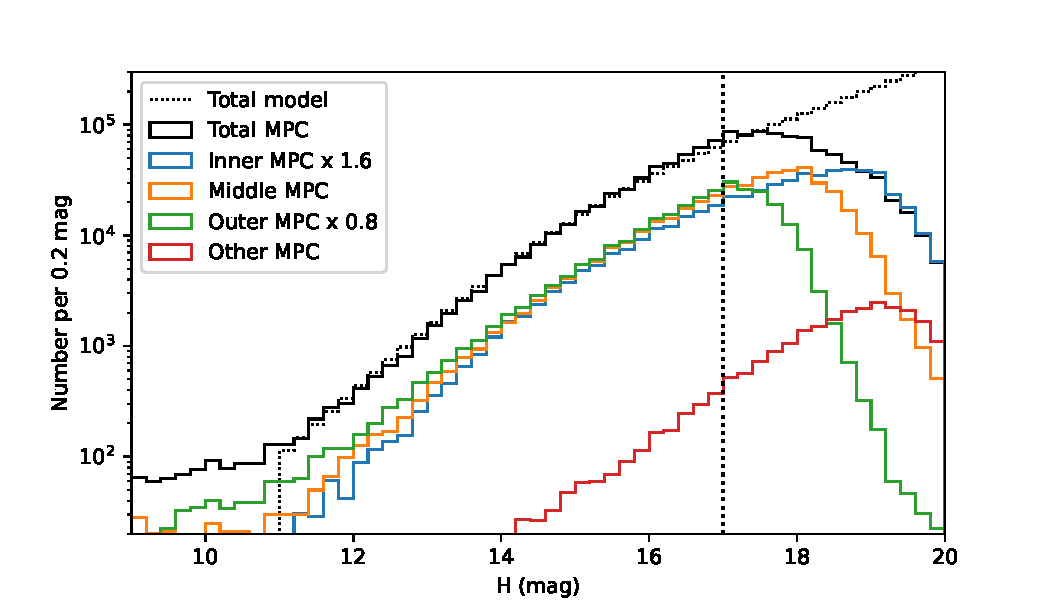
\includegraphics{mbacounts.pdf}
  \caption{Differential counts of MBAs cataloged by the MPC are
    plotted vs absolute magnitude $H$  
    for the Inner, Middle, Outer, and ``Other'' regions of
    the main belt, and for their total.  We assume that they are
    complete for $H\le17,$ and extrapolate to fainter sources using
    the functional form from \eqq{eq:lsstmba} shown as the dotted
    curve.}
  \label{fig:counts}
\end{figure}

Figure~\ref{fig:counts} plots our assumptions for $dN/dH.$  The MPC
catalog is likely close to complete in all three regions for $H\le17,$
so we will use the MPC counts directly in this regime.  Note that the
three regions have similar shapes of $dN/dH.$  For $H>17,$ we adopt
the functional form for the cumulative MBA counts given by
initial LSST predictions \citep{LSST_science_book}:
\begin{equation}
  N(<H) \propto \frac{10^{0.43(H-15.7)}}{10^{0.18(H-15.7)} +
    10^{-0.18(H-15.7)}},
\label{eq:lsstmba}
\end{equation}
normalizing this curve to the observed $H<17$ counts for each region.

\subsubsection{Individually detectable impulses}

\subsubsection{Results}


\section{Propagation to position shifts}
\label{sec:propagation}

\subsection{Element shifts from impulses}
\label{sec:elements}

Five of our orbital element perturbations $\vecq$ will be taken from constants of the motion.  The mean anomaly $M$ is not appropriate as the sixth, time-dependent element of $\vecq$ because the derivative $dM/dI$ can diverge as $e_0\rightarrow 0.$ Instead we introduce $\tau = M+\lop,$ which we will show does have a shift $\Delta\tau$ during an impulse that has finite and linear response to $\vecI$.  Between impulses, $\tau$ advances with the mean motion as $a^{-3/2}t.$  We define a coordinate system that is uniformly rotating with the unperturbed $\tau_0=t+M_0.$ The two smoothly rotating unit vectors $\uhat_\parallel=(\cos \tau_0, \sin \tau_0)$ and
$\uhat_\perp=(-\sin \tau_0, \cos \tau_0)$ satisfy $\uhat_\parallel \times \uhat_\perp = \zhat,$ and we will use subscripts $\parallel$ and $\perp$ to represent projections onto these components.  In particular, the components of the ellipticity vector $e_\parallel$ and $e_\perp$ have the values $e_\parallel=e\cos M$ and $e_\perp=-e\sin M$ in the unperturbed orbit.
The true anomaly $\nu,$ radius $r$, and azimuthal angle $\phi,$ and the velocity components of the initial orbit to $O(e)$ are
\begin{eqnarray}
  M & = & M_0 + t = \tau_0,  \nonumber \\
  \nu & = & M - 2 e_\perp \nonumber \\
  \phi & = & \nu + \lop = \tau - 2e_\perp, \nonumber\\
  r & = & 1-e_\parallel, \nonumber \\
  v_r & = & -e_\perp \nonumber \\
  v_t & = & 1 + e_\parallel
            \label{eq:kepler}
\end{eqnarray}

The first element adopted for $\vecq$ is the shift $\Delta a$, derivable from the orbital energy $E=-1/2a.$
\begin{eqnarray}
  \Delta E & = &  \vecv \cdot \vecI + O(I^2) \\
  \quad \Rightarrow \quad \Delta a & = & 2\left(v_r I_r + v_\phi I_\phi\right) = -2e_\perp I_r + 2(1+e_\parallel) I_\phi.
  \label{eq:da}
\end{eqnarray}
The initial angular momentum $\mathbf{L} = \sqrt{1-e^2}\,\zhat \approx \zhat$ is altered by
\begin{eqnarray}
  \Delta \mathbf{L} & = & \vecr \times \vecI = (1-e_\parallel) I_\phi \zhat - (1-e_\parallel) I_z \phat \\
  \quad \Rightarrow \quad \Delta \Lhat_\parallel & = & -2e_\perp I_z
  \label{eq:dLpar}\\
  \Delta \Lhat_\perp & = & -(1-e_\parallel)  I_z
                  \label{eq:dLperp}
\end{eqnarray}
We adopt the changes in direction $(\Delta\Lhat_x, \Delta\Lhat_y)$ as the next two elements of $\vecq$ specifying the inclination and ascending node $\Omega$ of the perturbed orbit.  These are a rotation of $(\Delta\Lhat_\parallel, \Delta\Lhat_\perp)$ by the angle $\tau.$  The conversion from the first line above to the subsequent two makes use of the decomposition $\phat=\uhat_\perp + 2e_\perp \uhat_\parallel$ derivable from the value of $\phi$ in Equations~(\ref{eq:kepler}).

The eccentricity vector $\vece = \vecv \times (\vecr \times \vecv) - \rhat$ is altered by the impulse according to
\begin{eqnarray}
  \Delta\vece & = & (2\rhat - rv_r \phat) I_t - \phat I_r \\
\label{eq:depar}
  \quad \Rightarrow \quad \Delta e_\parallel & = &  -2e_\perp I_r + 2 I_\phi \\
\Delta e_\perp & = & -I_r - 3e_\perp I_\phi.
\label{eq:deperp}
\end{eqnarray}
We adopt $\Delta e_x$ and $\Delta e_y$ as two additional components of $\vecq,$ again related through a rotation by $\tau$ to the quantities in Equations~(\ref{eq:depar}) and (\ref{eq:deperp}).

The final element of $\vecq$ will be the shift $\Delta\tau$ induced in $M+\lop$ by the impulse.  This can be obtained by enforcing the conditions that the radius $r$ or the azimuthal angle $\phi$ must remain constant during the impulse.  To findthe latter, we need a formula for $\nu(M)$ as a power series in $e.$  Standard formulae in the literature lead to:
\begin{eqnarray}
  \nu & = & M + 2e \sin M + \frac{5e^2}{4} \sin 2M + O(e^3) \\
  \label{eq:nue2}
    & = & M + 2(e\sin M) + \frac{5}{2} (e \sin M) (e \cos M) + O(e^3) 
\end{eqnarray}
We wish to find the first-order shift in $\phi=\nu + \lop$ and set it to zero.  But the derivatives of $M$ and $\lop$ with impulse can become infinite.  Instead we introduce a perturbation $\Delta\tau = \Delta(M+\lop).$ We can now express several post-impact quantities as deviations from the unperturbed quantities (subscripted with 0):
\begin{eqnarray}
  M & = & \tau-\lop = \tau_0 -\lop + \Delta\tau \\
  e \sin M & = & e \sin (\tau_0 -\lop) + \Delta\tau \left[ e \cos  (\tau_0 -\lop)\right] \\
    & = & -e_{0\perp}-\Delta e_\perp + e_{0\parallel} \Delta\tau +O(e^2) \\
  e \cos M & = & e \cos (\tau_0 -\lop) - \Delta\tau \left[ e \sin  (\tau_0 -\lop)\right] \\
    & = & e_{0\parallel}+\Delta e_\parallel + e_{0\perp} \Delta\tau +O(e^2) \\
\Rightarrow \quad \phi =\nu+\lop & = & \tau_0 + \Delta \tau + 2( -e_{0\perp}-\Delta e_\perp + e_{0\parallel} \Delta\tau )
                              + \frac{5}{2}\left( -e_{0\perp}\Delta e_\parallel-e_{0\parallel}\Delta e_\perp\right) + O(e^2).
\end{eqnarray}
Forcing $\phi$ to be unchanged during the impulse requires
\begin{eqnarray}
  \Delta\tau & = & \frac{5 e_\perp}{2} \Delta e_\parallel + \left(2-\frac{3e_\parallel}{2}\right) \Delta e_\perp \\
             & = & \left(-2+\frac{3e_\parallel}{2}\right) I_r - e_\perp I_\phi.
                   \label{eq:dtau0}
\end{eqnarray}
We have dropped the 0 subscripts on $e_\parallel,e_\perp$ at this point for brevity---they will refer to the values for the unperturbed orbit at the time of impulse, unless noted otherwise.

After the impulse, the mean anomaly $M$ advances at a rate of $a^{-3/2}t,$ meaning that an additional term $\Delta\tau = -3\Delta a (t-t_i)/2$ accrues by time $t$. The total perturbation of $\tau$ from the nominal value $t+M_0$ becomes
\begin{equation}
  \Delta\tau= \left[-2+\frac{3e_\parallel}{2} +3 e_\perp (t-t_i)\right] I_r  - \left[3(1+e_\parallel)(t-t_i) + e_\perp\right] I_\phi.
  \label{eq:dtau}
\end{equation}

This equation gives the last row of the $\matA$ matrix giving element-level perturbations from individual impulses.  The preceding equations can be restated to give the other rows:
\begin{eqnarray}
  \Delta a & = & -2e_\perp I_r + 2(1+e_\perp) I_\phi, \\
  \Delta \Lhat_\parallel & = & -2e_\perp I_z \\
  \Delta \Lhat_\perp & = & -(1-e_\parallel) I_z \\
  \Delta e_\parallel & = &  -2e_\perp I_r + 2 I_\phi \\
  \Delta e_\perp & = & -I_r - 3e_\perp I_\phi.
\end{eqnarray}

\subsection{Astrometric and ranging shifts from elements shifts}
\label{sec:observe}
\begin{equation}
  \label{eq:Ee2}
  \cos E  =  e\cos M - (e \sin M)^2 + O(e^3).
\end{equation}

Keeping only terms from Equations~(\ref{eq:kepler}) up to first order in $\vecq,$ the true anomaly $\nu,$ mean anomaly $M=t + \Delta t - \lop,$ and the azimuthal angle $\phi$ are related by
\begin{eqnarray}
  \nu  =  M + 2e\sin M  & = & t +  2e_0 \sin t  + \Delta t - \lop + 2 e_0(\Delta t - \lop) \cos t + 2\sin t \Delta e_x \\
  \Rightarrow \quad \phi  =  \nu + \lop & = &  \left[t + 2e_0\sin t\right] + \left[(1+2e_0\cos t) \Delta t - 2\cos t \Delta e_y + 2\sin t \Delta e_x\right]
                                                    \label{eq:phi}
\end{eqnarray}
where we have used $e_0\lop = \Delta e_y.$ The radial coordinate and polar angle $\theta$ are
\begin{eqnarray}
  r & = & (1 + \Delta a) \left[1- (e_0+\Delta e_x) \cos M \right] \nonumber \\
\label{eq:r}
  & = & \left[ 1-e_0\cos t \right] + \left[ (1-e_0\cos t) \Delta a + e_0\sin t \Delta t - \sin t \Delta e_y - \cos t \Delta e_x \right] \\
  \theta = z/r & = & -\Lhat_x \cos\phi - \Lhat_y \sin\phi \nonumber \\
\label{eq:theta}
               & = & \left[ 0 \right] + \left[ -\cos t \Lhat_x  - \sin t \Lhat_y\right].
\end{eqnarray}
The second line of each deviation is divided into two bracketed terms, the first being the initial orbit and the second being the first-order terms in elements of $\vecq,$ which are therefore the elements of $\matB$.

A heliocentric observer will measure ``range noise'' of $\covm^p_{rr}=\langle (\Delta r)^2\rangle$ in the measured distance to the target asteroid.  We find this by squaring the second bracketed term for $r$ and averaging $t$ over an interval of size $2\pi$ to compensate for the fact that we have assumed $M=0$ at $t=0,$ whereas in fact the $M_0$ values are random.  We can then derive
\begin{equation}
  \left\langle(\Delta r)^2\right\rangle = (\Delta a)^2 + \frac{1}{2}\left[ (\Delta e_x)^2 + (\Delta e_y)^2\right] + \frac{e_0}{2}(\Delta a \Delta e_x -  \Delta t \Delta e_y).
  \label{eq:varr}
\end{equation}
The same heliocentric observer will see angular shifts of the target position satisfying
\begin{eqnarray}
  \label{eq:phiphi}
  \left\langle (\Delta\phi)^2\right\rangle & = & (\Delta t)^2 + 2(\Delta e_x^2 + \Delta e_y^2)  -4e_0
  \left(\Delta t \Delta e_y\right)\\
  \label{eq:thetatheta}
  \left\langle (\Delta\theta)^2\right\rangle & = & \frac{1}{2} \left( \Lhat_x^2 + \Lhat_y^2\right) \\
  \label{eq:thetaphi}
  \left\langle \Delta\theta\Delta\phi\right\rangle & = & -e_0\Delta t \Lhat_x + (\Delta e_y \Lhat_x -  \Delta e_x \Lhat_y)
\end{eqnarray}

\section{Results and conclusions}
\label{sec:results}

\begin{acknowledgments}
  This work was supported by NSF grant AST-????.
  This research has made use of data and/or services provided by the International Astronomical Union's Minor Planet Center. 
\end{acknowledgments}

\newpage
\bibliographystyle{aasjournal}
%\bibliography{references}


\end{document}
